\documentclass{article}
\usepackage[hmargin=1in,vmargin=1.5in]{geometry}
\usepackage{amsmath}
\usepackage{amsfonts}
\usepackage{graphicx}
\usepackage{subcaption}
\usepackage{bm}
\newcommand{\x}{\bm x}
\title{Homework 4}
\setcounter{MaxMatrixCols}{20}
\author{Xinyi Gu, Songchen Tan}
\date{\today}
\begin{document}
\maketitle
\section{}
See the solution in Figure 1.
\begin{figure}[!ht]
    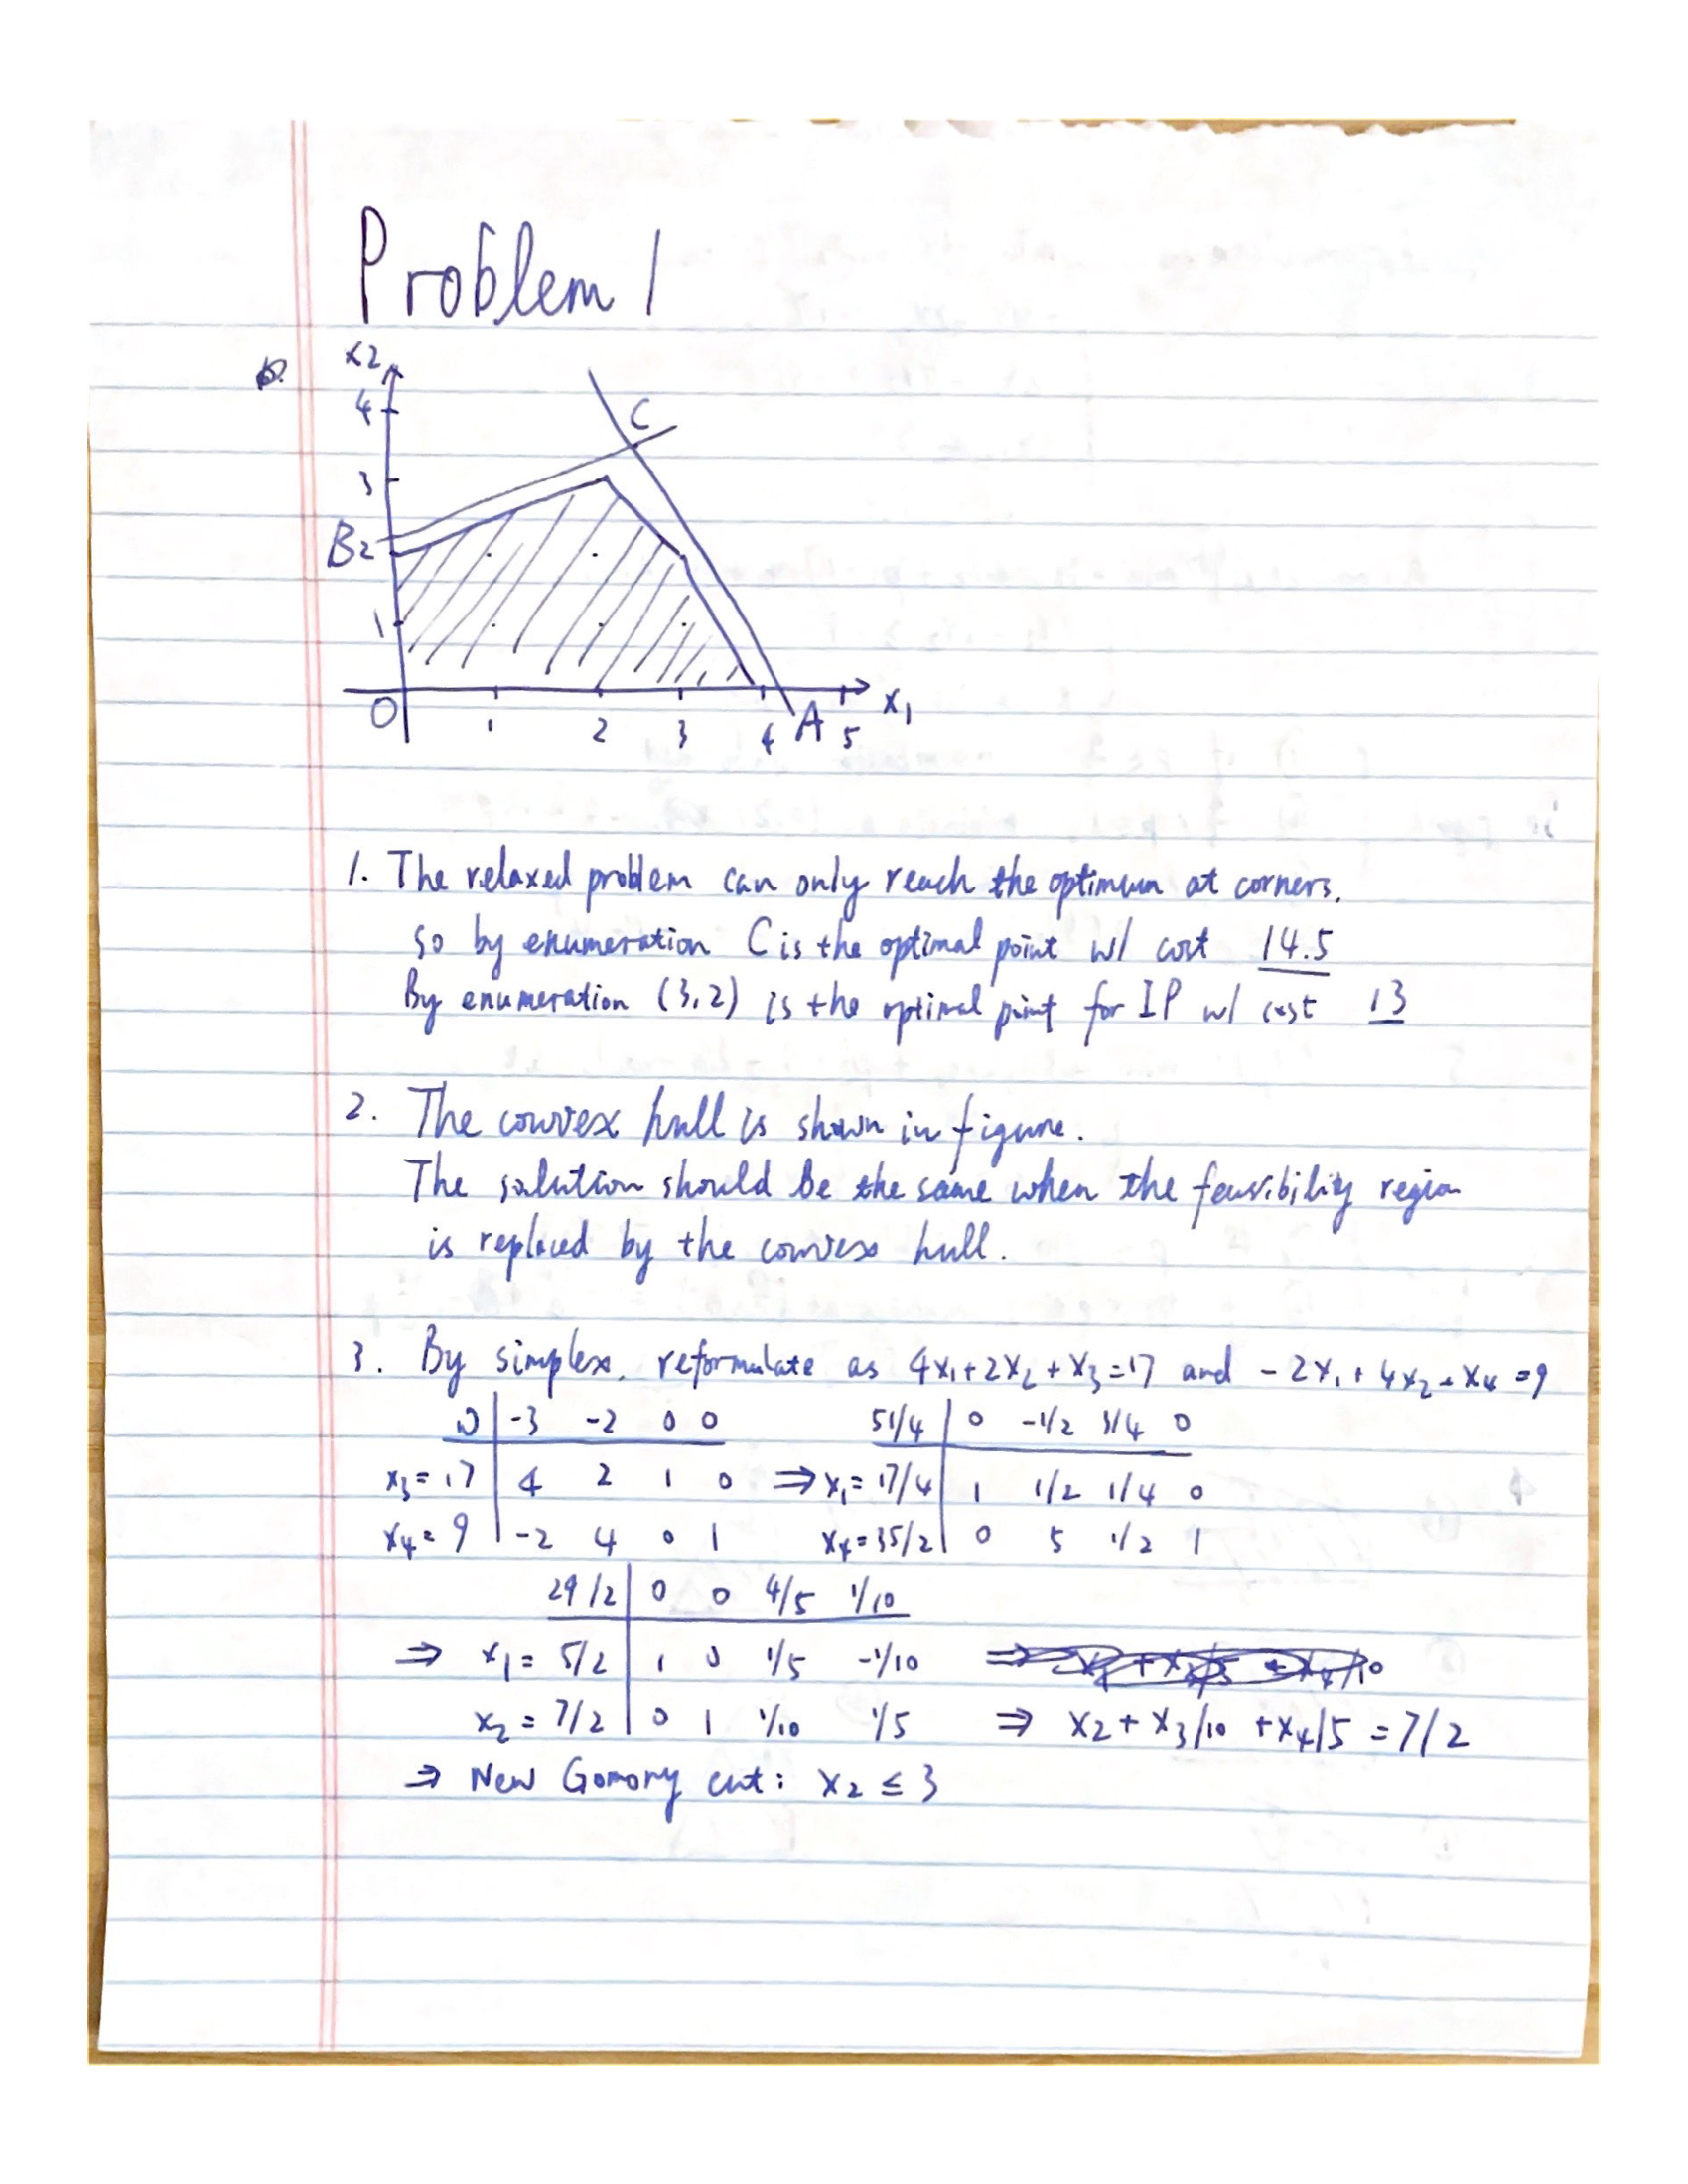
\includegraphics[width=\textwidth]{1.1.png}
\end{figure}
\begin{figure}[!ht]
    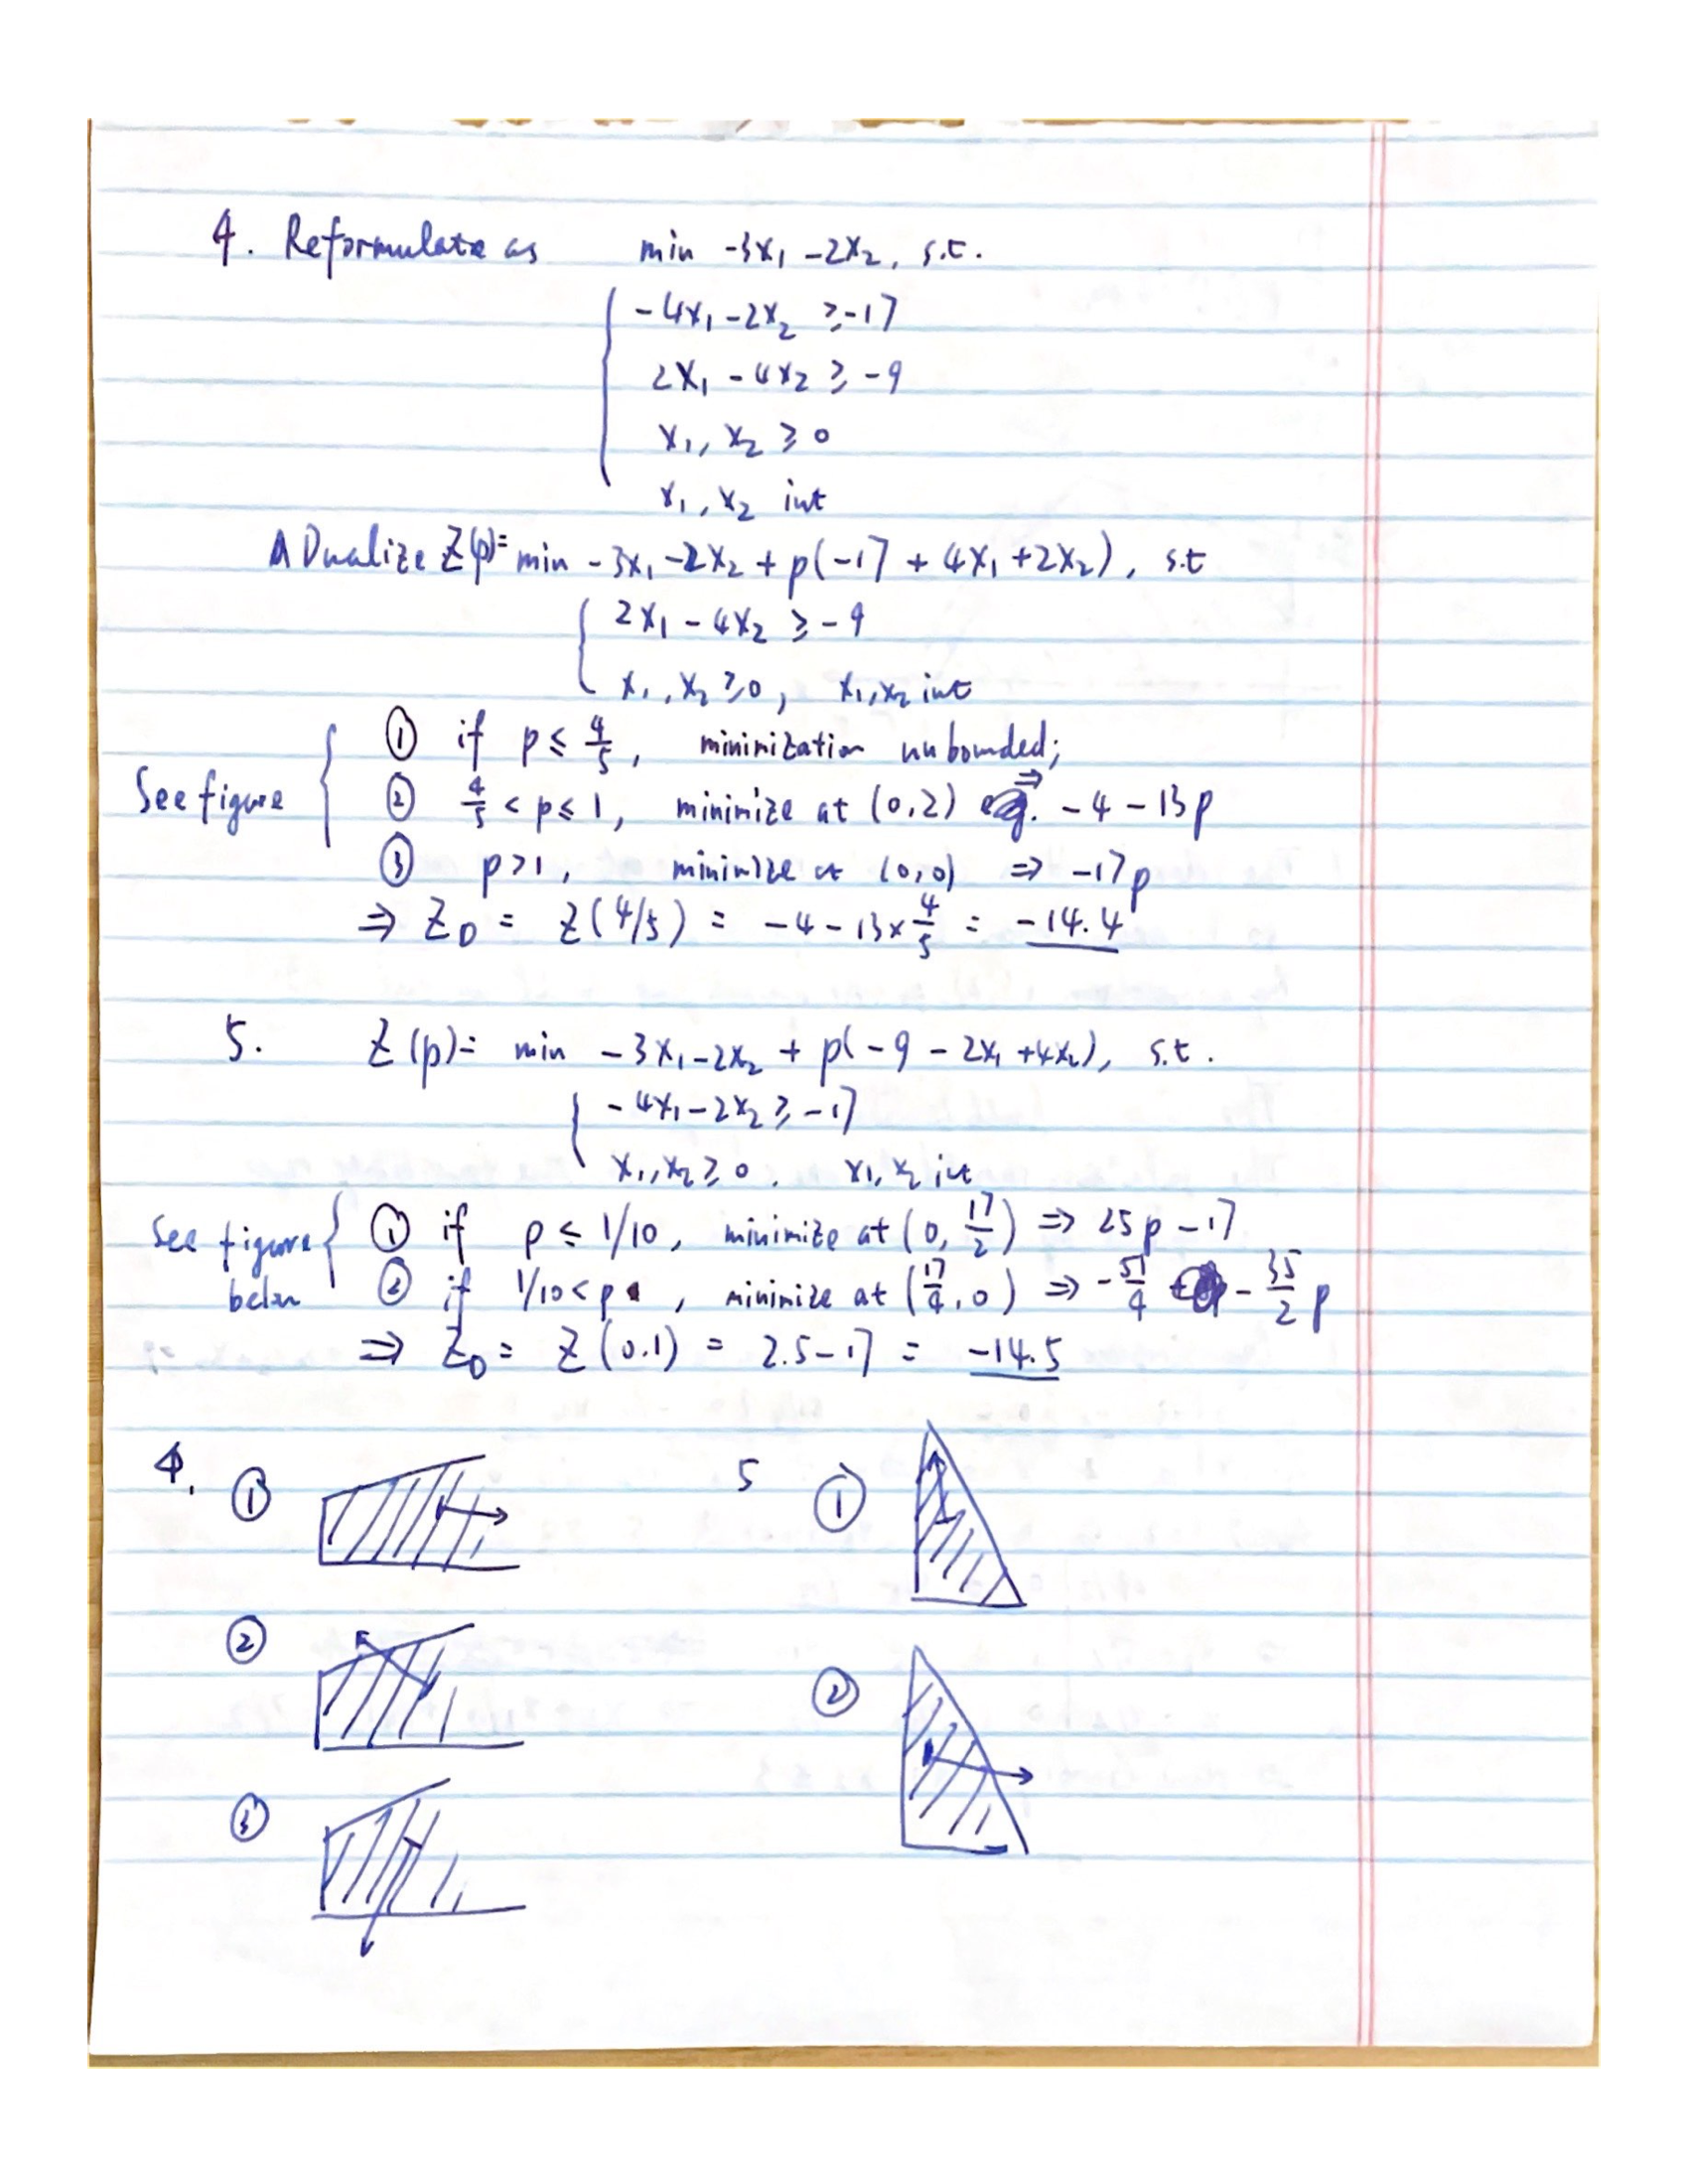
\includegraphics[width=\textwidth]{1.2.png}
    \caption{Solution to Problem 1}
\end{figure}
\section{}
\section{}
We denote the set defined by the first set, second set and third constraint to be $C_1,C_2,C_3$, and set $0\le x_{ij}\le 1$ to be $C_4$. Denoting the feasible set after four kinds of relaxations to be $X_1=C_1\cap C_2\cap C_4\cap\mathbb Z$, $X_2=C_3\cap C_4\cap\mathbb Z$, $X_3=C_2\cap C_3\cap C_4\cap\mathbb Z$, and $X_4=C_2\cap C_4\cap\mathbb Z$. Let $\x=\{x_{ij}\}$ $z=\sum_{ij}c_{ij}x_{ij}$, we have

\begin{itemize}
    \item $Z_{LP}=\min z$ s.t. $\x\in P_{LP}=C_1\cap C_2\cap C_3\cap C_4$;
    \item $Z_{D1}=\min z$ s.t. $\x\in P_1=C_3\cap \operatorname{CH}(X_1)$;
    \item $Z_{D2}=\min z$ s.t. $\x\in P_2=C_1\cap C_2\cap \operatorname{CH}(X_2)$;
    \item $Z_{D3}=\min z$ s.t. $\x\in P_3=C_1\cap \operatorname{CH}(X_3)$;
    \item $Z_{D4}=\min z$ s.t. $\x\in P_4=C_1\cap C_3\cap \operatorname{CH}(X_4)$;
    \item $Z_{IP}=\min z$ s.t. $\x\in P_{IP}=C_1\cap C_2\cap C_3\cap C_4\cap\mathbb Z$;
\end{itemize}

We first give a lemma on the property of convex hulls: if $A$ is a convex set and $B$ is an arbitrary set, then $\operatorname{CH}(A\cap B)$ is a subset of $A\cap\operatorname{CH}(B)$. This is because for any point in the former set, there exists a convex combination of points in $A\cap B$ that yields this point; and therefore this point is a member of both $\operatorname{CH}(B)$ and $\operatorname{CH}(A)$. Since $A=\operatorname{CH}(A)$, the point is a member of $A\cap\operatorname{CH}(B)$.


Using this lemma, we get $C_1\cap C_2\cap \operatorname{CH}(X_2)\subseteq C_1\cap C_2\cap C_3\cap \operatorname{CH}(C_4\cap\mathbb Z)=C_1\cap C_2\cap C_3\cap C_4$, therefore $P_2\subseteq P_{LP}$, so $Z_{LP}\le Z_{D2}$. Similarly, we can trivially get $Z_{D2}\le Z_{D3}\le Z_{IP}$.

When the third constraint is relaxed, the problem can be reformulated as a network flow problem, and the integrality of such problems implies that solving each subproblem $Z_{D1}(p)$ in $\operatorname{CH}(X_1)$ is equivalent to solving in $C_1\cap C_2\cap C_4$, therefore we have $Z_{D1}=Z_{LP}$. Similarly $Z_{D4}=Z_{LP}$. Assembling all the relationship we got so far gives us the desired order.

\section{}

\end{document}
